\documentclass[12pt]{article}
\usepackage[utf8]{inputenc}
\usepackage{amsmath}
\usepackage{graphicx}
\usepackage{multicol}
\usepackage{fancyhdr}

\usepackage[
    left=2.5cm,
    right=2.5cm,
    top=4cm,
    bottom=4cm
]{geometry}
\setlength{\parindent}{0em}

\setlength{\headheight}{15.0pt}
\pagestyle{fancy}
\lhead{18.06 Lectures 1-5}
\chead{Alisa Ono}
\rhead{January 2018}

\begin{document}

\section{The Geometry of Linear Equations (L1)}

\subsection{Example 1: 2 Unknowns}

\begin{multicols}{2}
{\[ 
\left \{
  \begin{tabular}{ccc}
  $2x$ & $-y$ &$= 0$ \\
  $-x$ & $+2y$ &$= 3$
  \end{tabular}
\right
.\]}

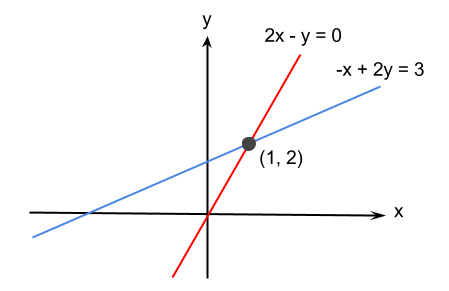
\includegraphics[width=\linewidth]{1-1}
\end{multicols}

The two lines intersect at (1,2) $\Rightarrow$ $x=1,y=2$ satisfy the two equations.

The equations represented in $Ax=b$ form:
\[
\left(
    \begin{matrix}
        2 & -1\\ 
        -1 & 2 
    \end{matrix}
\right)
\left(
    \begin{matrix}
        x\\ 
        y 
    \end{matrix}
\right)
=
\left(
    \begin{matrix}
        0\\ 
        3 
    \end{matrix}
\right)
\]

Represented as a linear combination of columns:
\begin{multicols}{2}
{\[
x
\left(
    \begin{matrix}
        2\\ 
        -1 
    \end{matrix}
\right)
+y
\left(
    \begin{matrix}
        -1\\ 
        2 
    \end{matrix}
\right)
=
\left(
    \begin{matrix}
        0\\ 
        3 
    \end{matrix}
\right)
\]}

\centering
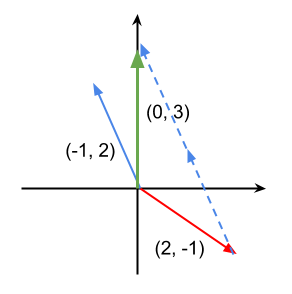
\includegraphics[width=0.6\linewidth]{1-2}
\end{multicols}

$x=1,y=2$ also satisfy the combination of columns.

\subsection{Example 2: 3 Unknowns}

\[ 
\left \{
  \begin{tabular}{cccc}
  $2x$ & $-y$ & & $=0$\\
  $-x$ & $+2y$ & $-z$ & $=-1$\\
  & $-3y$ & $+4z$ & $=4$\\
  \end{tabular}
\right
.\]

Each equation can be represented as a plane. The solution then is the point where three planes intersect.

$\>$

The equations represented in $Ax=b$ form:
\[
\left(
    \begin{matrix}
        2 & -1 & 0\\ 
        -1 & 2 & -1\\
        0 & -3 & 4
    \end{matrix}
\right)
\left(
    \begin{matrix}
        x\\ 
        y\\
        z\\
    \end{matrix}
\right)
=
\left(
    \begin{matrix}
        0\\ 
        -1\\
        4
    \end{matrix}
\right)
\]

Represented as a linear combination of columns:
\[
x
\left(
    \begin{matrix}
        2\\ 
        -1\\
        0
    \end{matrix}
\right)
+y
\left(
    \begin{matrix}
        -1\\ 
        2\\
        -3\\
    \end{matrix}
\right)
+z
\left(
    \begin{matrix}
        0\\ 
        -1\\
        4\\
    \end{matrix}
\right)
=
\left(
    \begin{matrix}
        0\\ 
        -1\\
        4
    \end{matrix}
\right)
\]

We can easily see that $x=0, y=0, z=1$ satisfy the combination of columns.

$\>$

Similarly, if we change the right hand side to:
\[
x
\left(
    \begin{matrix}
        2\\ 
        -1\\
        0
    \end{matrix}
\right)
+y
\left(
    \begin{matrix}
        -1\\ 
        2\\
        -3\\
    \end{matrix}
\right)
+z
\left(
    \begin{matrix}
        0\\ 
        -1\\
        4\\
    \end{matrix}
\right)
=
\left(
    \begin{matrix}
        1\\ 
        1\\
        -3
    \end{matrix}
\right)
\]

We can also easily see that $x=1, y=1, z=0$ satisfy the combination of columns.

\subsection{Solution Spaces}

Q. Given we have 3 unknowns, do the linear combinations of columns fill the 3-D space? i.e. Can we solve $Ax=b$ for any $b$?

$\>$

A. YES for the columns from the example above because the matrix is non-singular and invertible. NO if the column vectors lie on the same plane i.e. 2-D space.

$\>$

Q. How about 9 unknowns i.e. '9-D' space?

$\>$

A. NO if the column vector lie on the same '8-D' space.

\newpage

\section{Elimination with Matrices (L2)}

\subsection{Gaussian Elimination}

\[ 
\left \{
  \begin{tabular}{cccc}
  $x$ & $+2y$ & $+z$ & $=2$\\
  $3x$ & $+8y$ & $+z$ & $=12$\\
  & $4y$ & $+z$ & $=2$\\
  \end{tabular}
\right
.\]

When the equations are represented in $Ax=b$ form:
\[
A=
\left(
    \begin{matrix}
        1 & 2 & 1\\ 
        3 & 8 & 1\\
        0 & 4 & 1
    \end{matrix}
\right)
\]

First pivot is 1 at (1, 1). We want to multiply the first row by a multiplier and subtract from the second row so that 3 at (2, 1) becomes 0. Such multiplier is 3:
\[
\left(
    \begin{matrix}
        \boxed{1} & 2 & 1\\ 
        3 & 8 & 1\\
        0 & 4 & 1
    \end{matrix}
\right)
\Rightarrow
\left(
    \begin{matrix}
        \boxed{1} & 2 & 1\\ 
        1-3*1 & 8-3*2 & 1-3*1\\
        0 & 4 & 1
    \end{matrix}
\right)
=
\left(
    \begin{matrix}
        \boxed{1} & 2 & 1\\ 
        0 & 2 & -2\\
        0 & 4 & 1
    \end{matrix}
\right)
\]

Second pivot is 2 at (2, 2). We now want to multiply the second row by a multiplier and subtract from the third row so that 4 at (3, 2) becomes 0. Such multiplier is 2:
\[
\left(
    \begin{matrix}
        1 & 2 & 1\\ 
        0 & \boxed{2} & -2\\
        0 & 4 & 1
    \end{matrix}
\right)
\Rightarrow
\left(
    \begin{matrix}
        1 & 2 & 1\\ 
        0 & \boxed{2} & -2\\
        0-2*0 & 4-2*2 & 1-2*(-2)
    \end{matrix}
\right)
=
\left(
    \begin{matrix}
        1 & 2 & 1\\ 
        0 & \boxed{2} & -2\\
        0 & 0 & 5
    \end{matrix}
\right)
\]

Third pivot is 5 at (3,3):
\[
\left(
    \begin{matrix}
        1 & 2 & 1\\ 
        0 & 2 & -2\\
        0 & 0 & \boxed{5}
    \end{matrix}
\right)
=U
\]

$\>$

\textbf{Pivots cannot be 0.} 

$\>$

For example, if
\[
A=
\left(
    \begin{matrix}
        1 & 2 & 1\\ 
        3 & 6 & 1\\
        0 & 4 & 1
    \end{matrix}
\right)
\]

After subtracting three times the first row from the second row, the second pivot becomes 0:
\[
\left(
    \begin{matrix}
        1 & 2 & 1\\ 
        1-3*1 & 6-3*2 & 1-3*1\\
        0 & 4 & 1
    \end{matrix}
\right)
=
\left(
    \begin{matrix}
        1 & 2 & 1\\ 
        0 & \boxed{0} & -2\\
        0 & 4 & 1
    \end{matrix}
\right)
\]

We must switch the second and third rows before proceeding so 4 becomes the new pivot.

$\>$

Another example, if
\[
A=
\left(
    \begin{matrix}
        1 & 2 & 1\\ 
        3 & 8 & 1\\
        0 & 4 & -4
    \end{matrix}
\right)
\]

After subtracting three times the first row from the second row, then subtracting twice the second row from the third row, the third pivot becomes 0:
\[
\left(
    \begin{matrix}
        1 & 2 & 1\\ 
        0 & 2 & -2\\
        0-2*0 & 4-2*2 & -4-2*(-2)
    \end{matrix}
\right)
=
\left(
    \begin{matrix}
        1 & 2 & 1\\ 
        0 & 2 & -2\\
        0 & 0 & \boxed{0}
    \end{matrix}
\right)
\]

Elimination fails because we cannot switch the rows to make the third pivot non-zero.

\subsection{Back Substitution}
Augment the original matrix $A$ with $b$:
\[
\left(
    \begin{array}{c|c}
        A & b
    \end{array}
\right)
=
\left(
    \begin{array}{ccc|c}
        1 & 2 & 1 & 2\\ 
        3 & 8 & 1 & 12\\
        0 & 4 & 1 & 2
    \end{array}
\right)
\]

Perform Gaussian elimination:
\[
\left(
    \begin{array}{ccc|c}
        \boxed{1} & 2 & 1 & 2\\ 
        3 & 8 & 1 & 12\\
        0 & 4 & 1 & 2
    \end{array}
\right)
\Rightarrow
\left(
    \begin{array}{ccc|c}
        1 & 2 & 1 & 2\\ 
        3-3*1 & 8-3*2 & 1-3*1 & 12-3*2\\
        0 & 4 & 1 & 2
    \end{array}
\right)
=
\left(
    \begin{array}{ccc|c}
        1 & 2 & 1 & 2\\ 
        0 & \boxed{2} & -2 & 6\\
        0 & 4 & 1 & 2
    \end{array}
\right)
\]
\[
\Rightarrow
\left(
    \begin{array}{ccc|c}
        1 & 2 & 1 & 2\\ 
        0 & 2 & -2 & 6\\
        0-2*0 & 4-2*2 & 1-2*(-2) & 2-2*6
    \end{array}
\right)
=
\left(
    \begin{array}{ccc|c}
        1 & 2 & 1 & 2\\ 
        0 & 2 & -2 & 6\\
        0 & 0 & \boxed{5} & -10
    \end{array}
\right)
\]

$\>$

Now write down the rows as equations and solve the unknowns by substitutions:
\[ 
\left \{
  \begin{tabular}{cccc}
  $x$ & $+2y$ & $+z$ & $=2$\\
  & $2y$ & $-2z$ & $=6$\\
  & & $5z$ & $=-10$\\
  \end{tabular}
\right
.\Rightarrow
\left \{
  \begin{tabular}{cc}
  $x$ & $=2$\\
  $y$ & $=1$\\
  $z$ & $=-2$\\
  \end{tabular}
\right
.\]

\subsection{Elementary Matrices}

We will translate the elimination process into matrix operations.

\[
A=
\left(
    \begin{matrix}
        1 & 2 & 1\\ 
        3 & 8 & 1\\
        0 & 4 & 1
    \end{matrix}
\right)
\]

Subtracting three times the first row from the second:
\[
E_{21}=
\left(
    \begin{matrix}
        1 & 0 & 0\\ 
        \boxed{-3} & 1 & 0\\
        0 & 0 & 1
    \end{matrix}
\right)
\Rightarrow
E_{21}A
=
\left(
    \begin{matrix}
        1 & 2 & 1\\ 
        0 & 2 & -2\\
        0 & 4 & 1
    \end{matrix}
\right)
\]
\begin{itemize}
    \item First row of $E_{21}$ has 1 at its first column because the first row of $E_{21}A$ should be the same as the first row of $A$.
    \item Second row of $E_{21}$ has -3 at its first and 1 at its second column because the second row of $E_{21}A$ should be three times the first row of $A$ subtracted from the second row of $A$.
    \item First row of $E_{21}$ has 1 at its third column because the third row of $E_{21}A$ should be the same as the third row of $A$.
\end{itemize}

Similarly, subtracting twice the second row from the third:
\[
E_{32}=
\left(
    \begin{matrix}
        1 & 0 & 0\\ 
        0 & 1 & 0\\
        0 & \boxed{-2} & 1
    \end{matrix}
\right)
\Rightarrow
E_{32}(E_{21}A)
=
\left(
    \begin{matrix}
        1 & 2 & 1\\ 
        0 & 2 & -2\\
        0 & 0 & 5
    \end{matrix}
\right)
=U
\]

In summary, we found elementary matrices $E_{21}$ and $E_{32}$ such that $E_{32}E_{21}A = U$

\newpage

\section{Multiplication and Inverse Matrices (L3)}

\subsection{Matrix Multiplications}
\textbf{Matrix $\times$ Column $\Rightarrow$ Column}
\[
\left(
    \begin{matrix}
        - & - & -\\ 
        - & - & -\\
        - & - & -
    \end{matrix}
\right)
\left(
    \begin{matrix}
        x\\ 
        y\\
        z
    \end{matrix}
\right)
=
\left(
    \begin{matrix}
        x \times \text{1st column}\\ 
        y \times \text{2nd column}\\
        z \times \text{3rd column}
    \end{matrix}
\right)
\]

\textbf{Row $\times$ Matrix $\Rightarrow$ Row}
\[
\left(
    \begin{matrix}
        x & y & z
    \end{matrix}
\right)
\left(
    \begin{matrix}
        - & - & -\\ 
        - & - & -\\
        - & - & -
    \end{matrix}
\right)
=
\left(
    \begin{matrix}
        x \times \text{1st row} & 
        y \times \text{2nd row} &
        z \times \text{3rd row}
    \end{matrix}
\right)
\]

\textbf{A (m $\times$ n) $\times$ B (n $\times$ p) $\Rightarrow$ C (m $\times$ p)}
\[
\left(
    \begin{array}{*{3}{c}}
    \cline{1-3}
    \multicolumn{1}{|c}{-} & - & \multicolumn{1}{c|}{-}\\
    \cline{1-3}
    - & - & -
    \end{array}
\right)
\left(
    \begin{array}{*{2}{c}}
    \cline{1-1}
    \multicolumn{1}{|c|}{-} & -\\
    \multicolumn{1}{|c|}{-} & -\\
    \multicolumn{1}{|c|}{-} & -\\
    \cline{1-1}
    \end{array}
\right)  
=
\left(
    \begin{matrix}
        \boxed{-} & -\\ 
        - & -
    \end{matrix}
\right)
\]

\[
(i\text{-th row of A}) \times (j\text{-th column of B}) = \sum_{k=1}^{n}{a_{ik}b_{kj}} = C_{ij}
\]

\subsubsection{A $\times$ B by Columns}
Each column of C is a combination of A's columns.

\[
(\text{A})
\left(
    \begin{array}{*{2}{c}}
    \cline{1-1}
    \multicolumn{1}{|c|}{-} & -\\
    \multicolumn{1}{|c|}{-} & -\\
    \multicolumn{1}{|c|}{-} & -\\
    \cline{1-1}
    \end{array}
\right)  
=
\left(
    \begin{array}{*{2}{c}}
    \cline{1-1}
    \multicolumn{1}{|c|}{-} & -\\
    \multicolumn{1}{|c|}{-} & -\\
    \cline{1-1}
    \end{array}
\right)  
\]

\[
\text{A} \times (j\text{-th column of B}) = j\text{-th column of C}
\]

\subsubsection{A $\times$ B by Rows}
Each row of C is a combination of B's rows.

\[
\left(
    \begin{array}{*{3}{c}}
    \cline{1-3}
    \multicolumn{1}{|c}{-} & - & \multicolumn{1}{c|}{-}\\
    \cline{1-3}
    - & - & -
    \end{array}
\right)
(\text{B})
=
\left(
    \begin{array}{*{2}{c}}
    \cline{1-2}
    \multicolumn{1}{|c}{-} & \multicolumn{1}{c|}{-}\\
    \cline{1-2}
    - & -
    \end{array}
\right)
\]

\[
(i\text{-th row of A}) \times \text{B} = i\text{-th row of C}
\]

\subsubsection{A $\times$ B by Column-Row Pairs}
AB is the sum of ($j$-th column of A) $\times$ ($i$-th row of B)
\[
\left(
    \begin{matrix}
        a_{1j}\\
        a_{2j}
    \end{matrix}
\right)
\left(
    \begin{matrix}
        b_{i1} & b_{i2}
    \end{matrix}
\right)
=
\left(
    \begin{matrix}
        a_{1j}b_{i1} & a_{1j}b_{i2}\\
        a_{2j}b_{i1} & a_{2j}b_{i2}
    \end{matrix}
\right)
\]

\subsubsection{A $\times$ B by Blocks}
We can also divide matrices into blocks of smaller matrices to multiply them.
\[
\left(
    \begin{matrix}
        (A_1) & (A_2)\\
        (A_3) & (A_4)
    \end{matrix}
\right)
\left(
    \begin{matrix}
        (B_1) & (B_2)\\
        (B_3) & (B_4)
    \end{matrix}
\right)
=
\left(
    \begin{matrix}
        (A_1B_1+A_2B_3) & (A_1B_2+A_2B_4)\\
        (A_3B_1+A_4B_3) & (A_3B_2+A_4B_4)
    \end{matrix}
\right)
\]

\subsection{Matrix Inverses}
Given a square matrix $A$, its inverse $A^{-1}$ exists if $A$ is non-singular and invertible.
\[A^{-1}A = I = AA^{-1}\]

\textbf{Singular, non-invertible $A$:}
\begin{itemize}
    \item Determinant of $A$ is zero.
    \item There exists a non-zero vector $x$ such that $Ax=0$\\
    \\
    \textit{Proof by contradiction}: If $A^{-1}$ existed and $Ax=0$, $A^{-1}Ax=x=0$, but $x\neq0$
\end{itemize}
For example, 
$A=\left(
    \begin{matrix}
        1 & 3\\
        2 & 6
    \end{matrix}
\right)$
is singular and non-invertible.
$Ax=0$ when
$x=\left(
    \begin{matrix}
        3\\
        -1
    \end{matrix}
\right)$

\subsubsection{Finding $A^{-1}$ with Gauss-Jordan}
\[ 
  \begin{tabular}{cccc}
    $\left(
        \begin{matrix}
            1 & 3\\
            2 & 7
        \end{matrix}
    \right)$ &
    $\left(
        \begin{matrix}
            a & c\\
            b & d
        \end{matrix}
    \right)$ &
    $=$ & 
    $\left(
        \begin{matrix}
            1 & 0\\
            0 & 1
        \end{matrix}
    \right)$\\
    $A$ & $A^{-1}$ & & $I$
  \end{tabular}
\]

Augment the matrix $A$ with $I$:
\[
\left(
    \begin{array}{c|c}
        A & I
    \end{array}
\right)
=
\left(
    \begin{array}{cc|cc}
        1 & 3 & 1 & 0\\ 
        2 & 7 & 0 & 1
    \end{array}
\right)
\]
We will repeat eliminations until the left side becomes $I$, which is when the right side is $A^{-1}$. Subtract twice the first row from the second:
\[
\Rightarrow
\left(
    \begin{array}{cc|cc}
        1 & 3 & 1 & 0\\ 
        2-2*1 & 7-2*3 & 0-2*1 & 1-2*0
    \end{array}
\right)
=
\left(
    \begin{array}{cc|cc}
        1 & 3 & 1 & 0\\ 
        0 & 1 & -2 & 1
    \end{array}
\right)
\]
Subtract three times the second row from the first:
\[
\Rightarrow
\left(
    \begin{array}{cc|cc}
        1-3*0 & 3-3*1 & 1-3*(-2) & 0-3*1\\ 
        0 & 1 & -2 & 1
    \end{array}
\right)
=
\left(
    \begin{array}{cc|cc}
        1 & 0 & 7 & -3\\ 
        0 & 1 & -2 & 1
    \end{array}
\right)
\]
\[
A^{-1}=
\left(
    \begin{matrix}
        7 & -3\\
        -2 & 1
    \end{matrix}
\right)
\]

$\>$

\textbf{Why is the right side $A^{-1}$?}

As shown in L2, we can represent the eliminations with an elementary matrix $E$:
\[E
\left(
    \begin{array}{c|c}
        A & I
    \end{array}
\right)
=
\left(
    \begin{array}{c|c}
        I & ?
    \end{array}
\right)
\]

Since $EA=I$, $E=A^{-1}$ therefore $?=EI=E=A^{-1}$

\newpage

\section{Factorization into A = LU (L4)}

\subsection{Matrix Inverses}

\[
\begin{tabular}{cc}
    \text{Inverse of $A$:} & $A^{-1}A = I = AA^{-1}$\\[5pt]
    \text{Inverse of $AB$:} & $(AB)(B^{-1}A^{-1}) = I = (B^{-1}A^{-1})(AB)$
\end{tabular}
\]

\subsection{A = LU with a Single Elementary Matrix}
As show in L2, we can represent the elimination of $A$ into $U$ (upper triangular matrix) in term of an elementary matrix:
\[ 
  \begin{tabular}{cccc}
    $\left(
        \begin{matrix}
            1 & 0\\
            -4 & 1
        \end{matrix}
    \right)$ &
    $\left(
        \begin{matrix}
            2 & 1\\
            8 & 7
        \end{matrix}
    \right)$ &
    $=$ & 
    $\left(
        \begin{matrix}
            2 & 1\\
            0 & 3
        \end{matrix}
    \right)$\\
    $E_{21}$ & $A$ & & $U$
  \end{tabular}
\]
Multiply both sides with $E_{21}^{-1}$:
\[
  \begin{tabular}{cccc}
    $\left(
        \begin{matrix}
            2 & 1\\
            8 & 7
        \end{matrix}
    \right)$ &
    $=$ & 
    $\left(
        \begin{matrix}
            1 & 0\\
            4 & 1
        \end{matrix}
    \right)$ &
    $\left(
        \begin{matrix}
            2 & 1\\
            0 & 3
        \end{matrix}
    \right)$\\
    $A$ & & $E_{21}^{-1}$ & $U$
  \end{tabular}
\]
We have transformed $EA=U$ to $A=LU$, where $L$ is a lower triangular matrix.
\[
L=
\left(
    \begin{matrix}
        1 & 0\\
        4 & 1
    \end{matrix}
\right)
\]

\subsection{A = LU with Multiple Elementary Matrices}

Assuming no row exchanges took place:

\[E_{32}E_{21}A = U\]
\[(E_{32}E_{21})^{-1} = E_{21}^{-1}E_{32}^{-1}\] 
\[A = E_{21}^{-1}E_{32}^{-1}U \Rightarrow L = E_{21}^{-1}E_{32}^{-1}\]

For example,
\[
E_{32}=
\left(
    \begin{matrix}
        1 & 0 & 0\\
        0 & 1 & 0\\
        0 & -5 & 1
    \end{matrix}
\right)
\quad
E_{21}=
\left(
    \begin{matrix}
        1 & 0 & 0\\
        -2 & 1 & 0\\
        0 & 0 & 1
    \end{matrix}
\right)
\]
\[
  \begin{tabular}{cccc}
    $\left(
        \begin{matrix}
            1 & 0 & 0\\
            0 & 1 & 0\\
            0 & -5 & 1
        \end{matrix}
    \right)$ &
    $\left(
        \begin{matrix}
            1 & 0 & 0\\
            -2 & 1 & 0\\
            0 & 0 & 1
        \end{matrix}
    \right)$ &
    $=$ & 
    $\left(
        \begin{matrix}
            1 & 0 & 0\\
            2 & 1 & 0\\
            0 & 5 & 1
        \end{matrix}
    \right)$\\
    $E_{21}^{-1}$ & $E_{32}^{-1}$ & & $L$
  \end{tabular}
\]

We can also see above that the multipliers, 5 for $E_{32}$ and 2 for $E_{21}$, go directly into $L$.

\subsection{Runtime of Elimination}
Given a $n\times{n}$ matrix $A$, how many operations (multiplication and subtraction) does it take to transform $A$ to $U$? Assume no row exchanges.

$\>$

It takes about $n^2$ operations to zero out the first column below the first pivot, $(n-1)^2$ for the second column below the second pivot, and so on...

\[n^2+(n-1)^2+...+1^2\approx{\frac{1}{3}n^3}\]

\newpage

\section{Transposes, Permutations, Spaces $R^n$ (L5)}

\subsection{Permutations}
Row exchanges can be represented as matrix operations with permutation matrix $P$.

$\>$

2$\times$2 matrix for example:
\[
\begin{tabular}{cccc}
    $\left(
        \begin{matrix}
            0 & 1\\
            1 & 0
        \end{matrix}
    \right)$ &
    $\left(
        \begin{matrix}
            a & b\\
            c & d
        \end{matrix}
    \right)$ &
    $=$ &
    $\left(
        \begin{matrix}
            c & d\\
            a & b
        \end{matrix}
    \right)$\\
    $P$ & & &
  \end{tabular}
\]

$P$ is an identity matrix with reordered rows. Below are all possible 3$\times$3 permutation matrices:

\[
\left(
    \begin{matrix}
        1 & 0 & 0\\
        0 & 1 & 0\\
        0 & 0 & 1\\
    \end{matrix}
\right)
\left(
    \begin{matrix}
        0 & 1 & 0\\
        1 & 0 & 0\\
        0 & 0 & 1\\
    \end{matrix}
\right)
\left(
    \begin{matrix}
        0 & 0 & 1\\
        0 & 1 & 0\\
        1 & 0 & 0\\
    \end{matrix}
\right)
\left(
    \begin{matrix}
        1 & 0 & 0\\
        0 & 0 & 1\\
        0 & 1 & 0\\
    \end{matrix}
\right)
\left(
    \begin{matrix}
        0 & 1 & 0\\
        0 & 0 & 1\\
        1 & 0 & 0\\
    \end{matrix}
\right)
\left(
    \begin{matrix}
        0 & 0 & 1\\
        1 & 0 & 0\\
        0 & 1 & 0\\
    \end{matrix}
\right)
\]

$\>$

There are $3!$ possible orderings for a 3$\times$3 identity matrix, thus 6 different 3$\times$3 permutation matrices. In general, there are $n!$ possible orderings for a $n\times{n}$ identity matrix, thus $n!$ different $n\times{n}$ permutation matrices.

$\>$

To account for the row exchanges, we can rewrite $A=LU$ as $PA=LU$.

\subsection{Transposes}

\[
    (A^T)_{ij}=Aji
\]

\[
\text{For example:}
\quad
A^T=
\left(
    \begin{matrix}
        1 & 3\\
        2 & 3\\
        4 & 1\\
    \end{matrix}
\right)^T
=
\left(
    \begin{matrix}
        1 & 2 & 4\\
        3 & 3 & 1\\
    \end{matrix}
\right)
\]

\textbf{Transposes of permutation matrices}
\[P^T = P^{-1} \quad \text{i.e.} \quad P^TP = I\]

\textbf{Inverse of transposes}
\[A^T(A^{-1})^T = I = (A^{-1})^TA^T\]

\subsubsection{Symmetric Matrices}

$A$ is symmetric if $A^T=A$. 

$\>$

$A^TA$ always produces a symmetric matrix because $(A^TA)^T = A^TA^{TT} = A^TA$

\[
\left(
    \begin{matrix}
        1 & 3\\
        2 & 3\\
        4 & 1\\
    \end{matrix}
\right)
\left(
    \begin{matrix}
        1 & 2 & 4\\
        3 & 3 & 1\\
    \end{matrix}
\right)
=
\left(
    \begin{matrix}
        10 & 11 & 7\\
        11 & 13 & 11\\
        7 & 11 & 17\\
    \end{matrix}
\right)
\]

\subsection{Vector Spaces}

Vector space $R^n$ represents all the $n$-dimensional real vectors i.e. all column vectors with $n$ real components.

$\>$

For example, $R^2$ represents all the 2-dimensional real vectors i.e. x-y plane. All column vectors that consist of 2 components such as 
$\left(
    \begin{matrix}
        3\\
        2 
    \end{matrix}
\right)$,
$\left(
    \begin{matrix}
        0\\
        0 
    \end{matrix}
\right)$,
$\left(
    \begin{matrix}
        \pi\\
        e 
    \end{matrix}
\right)$
are all part of $R^2$.

\subsubsection{Vector Subspaces}
Subspaces are vector spaces inside of $R^n$.

$\>$

If a vector space contains vectors $v$ and $w$, then it must also contain $cv+dw$ for any combinations of $c$ and $d$. This means that every vector space must contain the zero vector ($c=0, d=0$).

$\>$

\begin{multicols}{2}
For example, a subspace of $R^2$ is either:
\begin{itemize}
    \item All of $R^2$
    \item Line through the origin
    \item Only the vector $\left(\begin{matrix}0\\0\end{matrix}\right)$ i.e. $Z$
\end{itemize}

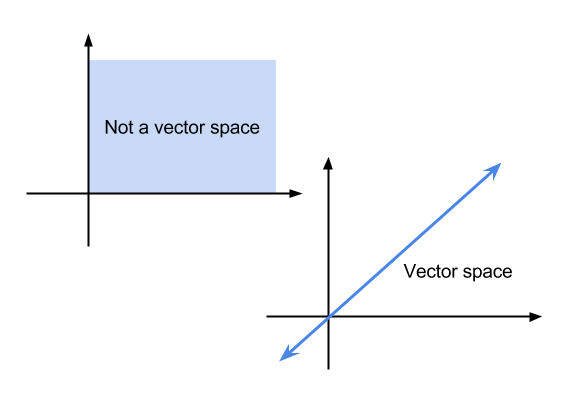
\includegraphics[width=\linewidth]{5-1}
\end{multicols}

\textbf{Combination of Subspaces}

$\>$

Given $P$ is a plane through the origin and $L$ is a line through the origin, $P$ and $L$ are both subspaces of $R^3$. 

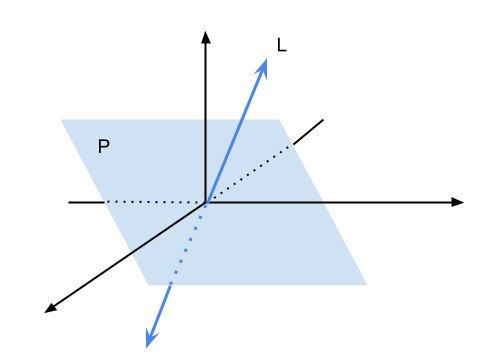
\includegraphics[width=0.7\linewidth]{5-2}

$P\cup{L}$ \underline{is not a subspace} of $R^3$, but $P\cap{L}$ i.e. the zero vector \underline{is a subspace} of $R^3$.

$\>$

In general, the intersection of two subspaces $S\cap{T}$ is also a subspace.

\end{document}
